\documentclass{article}

\usepackage{amsmath}
\usepackage{amssymb}
\usepackage{amsthm}
\usepackage{array}
\usepackage{geometry}
\usepackage{graphicx}
\usepackage{semantic}

\newcommand{\at}{\ensuremath{{\scriptstyle{@}}}}
\newcommand{\pc}{\ensuremath{{\mathit{pc}}}}

\newcommand{\twoheadlongmapsto}{\mapstochar\relbar\joinrel\twoheadrightarrow}

\renewcommand*\descriptionlabel[1]{\hspace\labelsep\normalfont #1}

\newcommand{\CoqSymbol}{\raisebox{-.2ex}{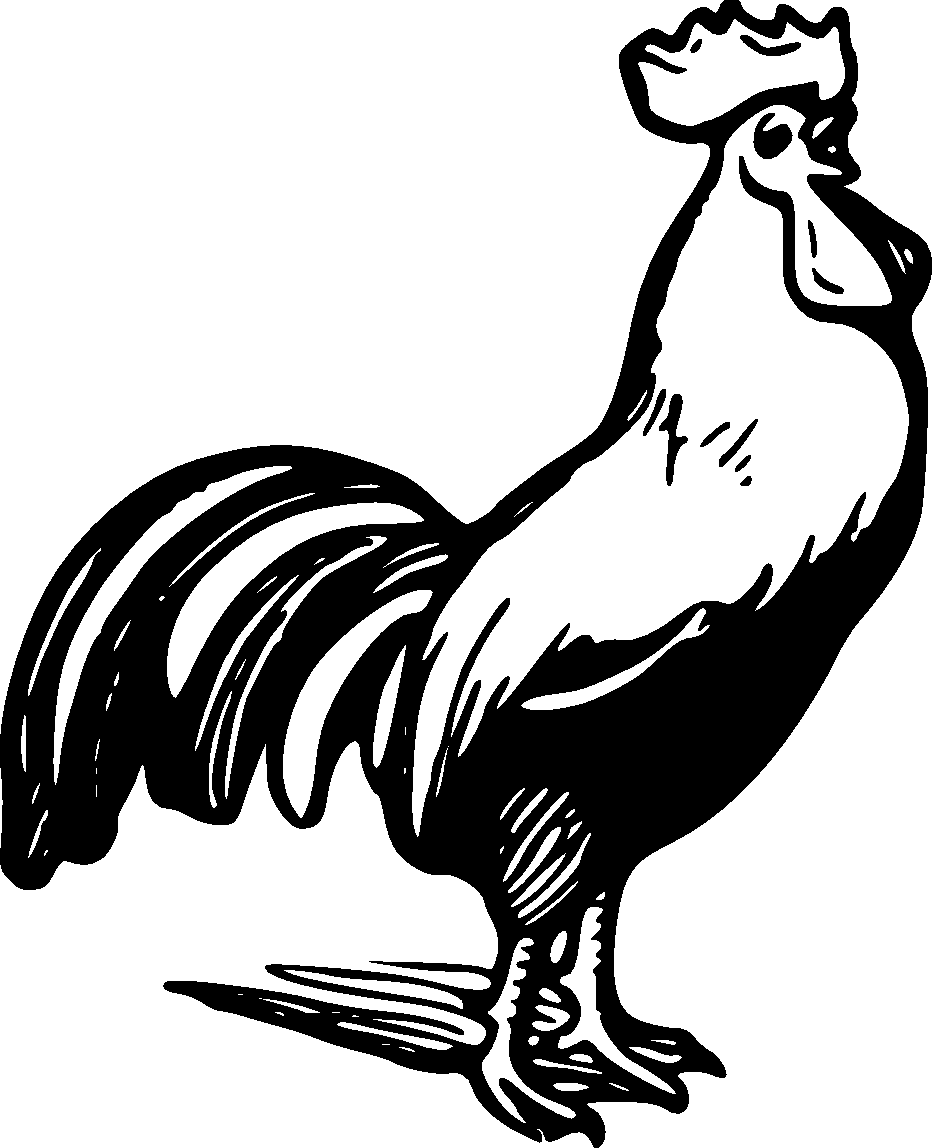
\includegraphics[height=0.9em]{coq.pdf}}\,}
\newcommand{\Coqed}{\hfill\CoqSymbol}

\theoremstyle{definition}
\newtheorem{theorem}{Theorem}
\newtheorem{lemma}{Lemma}
\newtheorem{definition}{Definition}

\begin{document}

\begin{flushright}
  %\texttt{github.com/esilkensen/auth}
  %\\
  \today
\end{flushright}

\begin{figure}[h]
  \centering
  \[
  \mathcal{L} = \{ \bot, \top \}
  \qquad
  \bot \sqsubseteq \top
  \qquad
  L^{\mathit{def}} = \bot
  \qquad
  \mathcal{A} = \mathbf{1}
  \]
  \caption{Label algebra $\mathbf{2}$.}
  \label{fig:two}
\end{figure}

\begin{figure}[h]
  \centering
  \[
  \begin{array}[t]{r @{\ } c @{\ } l c l}
    e & \in & \mathit{Exp} & ::= &
    n\;\; |\;\;
    x\;\; |\;\;
    \lambda{x}.\, e\;\; |\;\;
    e\ e\;\; |\;\;
    e \updownarrow_{A} %L
    \\[0.6ex]
    v & \in & \mathit{Val} & ::= &
    n\;\; |\;\;
    \langle{\rho, \lambda{x}.\, e\rangle}
    \\[0.6ex]
    a & \in & \mathit{Atom} & ::= &
    v \at L
    \\[0.6ex]
    \rho & \in & \mathit{Env} & ::= &
    \bullet\;\; |\;\;
    \rho, x = a
    \\[1.6ex]
    n & \in & \mathbb{N} & &
    \text{the set of natural numbers}
    \\[0.6ex]
    x & \in & \mathit{Var} & &
    \text{a set of identifiers}
  \end{array}
  \]
  \caption{Syntax of $\lambda_{\mathbf{2}}$.}
  \label{fig:syntax}
\end{figure}

\begin{figure}[h]
  \centering
  \begin{gather*}
    \inference{}{
      \pc, \rho |- n \Downarrow n \at \pc
    }[\textsc{E-Nat}]
    \qquad
    \inference{
      \rho(x) = v \at L
    }{
      \pc, \rho |- x \Downarrow v \at (\pc \sqcup L)
    }[\textsc{E-Var}]
    \\[6ex]
    \inference{}{
      \pc, \rho |- (\lambda{x}.\, e) \Downarrow
      \langle{\rho, \lambda{x}.\, e\rangle} \at \pc
    }[\textsc{E-Abs}]
    \qquad
    \inference{
      \pc, \rho |- e_1 \Downarrow
      \langle{\rho_1, \lambda{x}.\, e\rangle} \at L_1
      \\
      \pc, \rho |- e_2 \Downarrow a_2
      \\
      L_1, (\rho_1, x = a_2) |- e \Downarrow a_3
    }{
      \pc, \rho |- (e_1\ e_2) \Downarrow a_3
    }[\textsc{E-App}]
    \\[6ex]
    % \inference{
    %   \pc, \rho |- e_1 \Downarrow v_1 \at L_2
    %   \\
    %   L_1 \sqsubseteq_{A} L_2
    % }{
    %   \pc, \rho |- e_1 \updownarrow_{A} L_2
    % }[\textsc{E-Relabel}]
    \inference{
      \pc, \rho |- e \Downarrow v \at \bot
    }{
      \pc, \rho |- e \updownarrow_{A}\; \Downarrow v \at \bot
    }[\textsc{E-Relabel1}]
    \qquad
    \inference{
      \pc, \rho |- e \Downarrow v \at \top
      &
      \textit{Condition on } e
    }{
      \pc, \rho |- e \updownarrow_{A}\; \Downarrow v \at \bot
    }[\textsc{E-Relabel2}]
  \end{gather*}
  \caption{Semantics of $\lambda_{\mathbf{2}}$.}
  \label{fig:semantics}
\end{figure}

\pagebreak

\begin{definition}
  The $\approx^{L}_{P}$ relation expresses the \emph{indistinguishability} of
  atoms for observers at label $L$ and with respect to some reflexive predicate
  $P$, where $v_1 \at L_1 \approx^{L}_{P} v_2 \at L_2$ iff either
  \begin{itemize}
  \item $L = \bot$ and
    $L_1 = L_2 = \top$ and either
    \begin{itemize}
    \item $v_1 = n_1$ and
      $v_2 = n_2$ and
      $P(n_1, n_2)$, or
    \item $v_1 \not= n_1$ or $v_2 \not= n_2$; or
    \end{itemize}
  \item $L = \bot$ and
    $L_1 = L_2 = \bot$ and $v_1 \approx^{L}_{P} v_2$; or
  \item $L = \top$ and $L_1 = L_2$ and $v_1 \approx^{L}_{P} v_2$.
  \end{itemize}
  The definition for atoms is mutually recursive with that for values and
  environments:
  \begin{itemize}
  \item $n_1 \approx^{L}_{P} n_2$ iff $n_1 = n_2$.
  \item
    $\langle{\rho_1, \lambda{x_1}.\, e_1\rangle} \approx^{L}_{P}
    \langle{\rho_2, \lambda{x_2}.\, e_2\rangle}$ iff
    $\rho_1 \approx^{L}_{P} \rho_2$ and
    $\lambda{x_1}.\, e_1 \equiv \lambda{x_2}.\, e_2$.
  \item $\rho_1 \approx^{L}_{P} \rho_2$ iff
    $\mathrm{dom}\; \rho_1 = \mathrm{dom}\; \rho_2$ and
    $\rho_1(x) \approx^{L}_{P} \rho_2(x)$ for every
    $x \in \mathrm{dom}\; \rho_1$.
  \end{itemize}
  \label{def:indistinguishability}
\end{definition}

\begin{lemma}
  If $v_1 \at L_1 \approx^{L}_{P} v_2 \at L_2$, then $L_1 = L_2$.
  \Coqed
  \label{lem:lab-inversion}
\end{lemma}

\begin{lemma}
  If $v_1 \at \bot \approx^{L}_{P} v_2 \at \bot$, then
  $v_1 \at \top \approx^{L}_{P} v_2 \at \top$.
  \Coqed
  \label{lem:lab-raise}
\end{lemma}

\begin{lemma}
  If $\pc, \rho |- e \Downarrow v \at L$, then $pc \sqsubseteq L$.
  \Coqed
  \label{lem:eval-pc-lb}
\end{lemma}

\begin{theorem}
  If $\pc, \rho_1 |- e \Downarrow a_1$ and $\pc, \rho_2 |- e \Downarrow a_2$
  and $\rho_1 \approx^{L}_{P} \rho_2$, then $a_1 \approx^{L}_{P} a_2$.
\end{theorem}
\begin{proof}
  By induction on the derivation of $\pc, \rho_1 |- e \Downarrow a_1$.

    For the \textsc{E-App} case, by inversion $e = (e_1\ e_2)$ and:
    \begin{itemize}
    \item
      $\pc, \rho_1 |- e_1 \Downarrow
      \langle{\rho_{11}, \lambda{x_1}.\, e_{11}\rangle} \at L_{11}$
      \quad and \quad
      $\pc, \rho_2 |- e_1 \Downarrow
      \langle{\rho_{21}, \lambda{x_2}.\, e_{21}\rangle} \at L_{21}$
    \item
      $\pc, \rho_1 |- e_2 \Downarrow a_{12}$
      \hspace{17.2ex} and \quad
      $\pc, \rho_2 |- e_2 \Downarrow a_{22}$
    \item
      $L_{11}, (\rho_{11}, x_1 = a_{12}) |- e_{11} \Downarrow a_{13}$
      \hspace{2.54ex} and \quad
      $L_{21}, (\rho_{21}, x_2 = a_{22}) |- e_{21} \Downarrow a_{23}$
    \end{itemize}
    By the induction hypothesis,
    \begin{itemize}
    \item
      $\langle{\rho_{11}, \lambda{x_1}.\, e_{11}\rangle} \at L_{11}
      \approx^{L}_{P}
      \langle{\rho_{21}, \lambda{x_2}.\, e_{21}\rangle} \at L_{21}$
      \quad and \quad
      $a_{12} \approx^{L}_{P} a_{22}$
    \end{itemize}
    If we can show that
    \begin{itemize}
    \item 
      $L_{11} = L_{21}$
      \quad and \quad
      $(\rho_{11}, x_1 = a_{12}) \approx^{L}_{P} (\rho_{21}, x_2 = a_{22})$
      \quad and \quad
      $e_{11} = e_{21}$
    \end{itemize}
    then $a_{13} \approx^{L}_{P} a_{23}$ follows from the induction hypothesis,
    and the case is completed.
    
    However, we can't show that
    $(\rho_{11}, x_1 = a_{12}) \approx^{L}_{P} (\rho_{21}, x_2 = a_{22})$
    or that
    $e_{11} = e_{21}$, for example, when $L_{11} = L_{21} = \top$ and $L = \bot$,
    so the proof fails.
\end{proof}

\begin{flushleft}
  Questions:
\end{flushleft}

\begin{itemize}
\item Definition of \textsc{E-Relabel}.
\item Change definition of $\approx^{L}_{P}$? Change statement of theorem?
\item What properties should $P$ have? Should it be reflexive?
\item Should $\approx^{L}_{P}$ be an equivalence relation?
\item Should $a_1 \approx^{\top}_{P} a_2$ imply $a_1 \approx^{\bot}_{P} a_2$?
\end{itemize}

\end{document}
